\section{Implementation}
\label{sec.implementation}
\noindent The first step towards establishing the technologies which are most suited for this project, was to draw a high level architecture of the system. As the system is a lot about user interaction (i.e. presentation layer) we decided to go for a concrete separation between the domain~logic and the user~interface; the way to go in order to achieve this separation in a web application is by relying on the n-Tier architectural pattern. As we also need a persistent~storage which should also be separated by the domain-login and user-interface, we notice that our application is structured intothree layers. Hence, we are dealing with a system leveraging the 3-Tier\footnote{\url{http://en.wikipedia.org/wiki/Multitier_architecture}} architectural pattern, depicted in Figure\ref{fig.setup}.
\begin{figure}[H] 
	\centering
	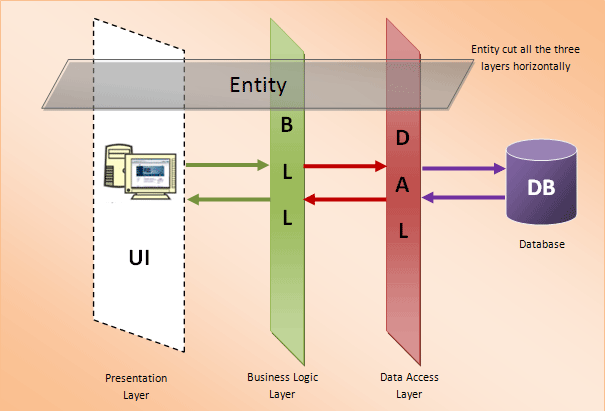
\includegraphics[width=\linewidth]{fig/3tier2}
	\caption{Concept of the 3-Tier Architectural pattern}
	\label{fig.setup}
\end{figure}
\\

\noindent Analysing the concept, we can see that it helps the application to separate the input~logic, business~logic and UI~logic, while providing a loose coupling between these elements. This allows for independent development, testing and maintenance of each component - called separation~of~concerns.
\\

\noindent Researching the frameworks that can help us carry out the current work, we have found a few suitable candidates: Apache~Struts, ASP.Net and Java~Server~Faces (JSF). When choosing the framework to use, we had to take into consideration the following constraints:
\begin{itemize}
  \item the framework has to be free and open-source; free, because we do not
  have a budget to buy software and open-source because this is an academic
  project and should promote open-source
  \item we have an account on an ITU server to deploy the system; this
  server runs a Unix-like operating system; hence the framework should run on
  Unix-like platforms
\end{itemize}
\\

\noindent ASP.Net is a web application framework, developed by Microsoft. We have excluded this candidate because it fails to adhere to both constraints listed above; it is not open-source and runs only on the Microsoft Windows platform.
\\

\noindent Apache Struts is an open-source web application framework helping to develop Java EE web applications. It is based on the Java Servlet API, encouraging the use of MVC architecture. This framework satisfies both constraints, but it is a rather old technology, supporting Java~Server~Pages (JSP) for the presentation layer.
\\

\noindent We wanted to go for something more fresh, choosing JSF~2 as the framework to base our development upon. JSF is a Java-based web application framework which simplifies the development integration of web-based user interfaces. The core features, together with the help they offer for our development process, are listed bellow, as summarized by \cite{wiki}. We have leared the basics of JSF2 using \cite{Geary:3}.
\begin{itemize}
  \item managed beans (a dependency~injection system) -- helps to easily manage the creation and injection of objects the system depends upon
  \item built in ajax support -- useful for dynamic form validations
  \item integration with the Unified Expression Language (EL), which represent the core function of JSF; views may access managed bean fields and methods via EL
  \item a default set of HTML and web-application specific UI components -- to easily create good-looking and complex pages
  \item state management, supporting: "request'', "session'' and "application' 'scoped Java beans -- helps to easily manage the lifetime of the managed beans.
\end{itemize}
\\

\noindent A JSF application needs to be deployed in an environment that is a web~server and which provides a servlet~container; although there are many options (JBoss, Glassfish etc.) we chose the simplest, Apache Tomcat 7, which is a lightweight open source web server and servlet container.
\\

\noindent Moreover, to build a robust and safe system in such a short period of time, we had to look for frameworks that can ease the development process in the main areas of the project: presentation, business and data access.
\\

\paragraph{In the data access layer} the development can become a lot easier having entities (classes) representing equivalents of the tables in the database. This is an important aspect, as it is a lot easier to interact with the database in an Object-Oriented (OO) manner, from code written in an OO language, by invoking operations on objects, than to write queries against the database. For this purpose we chose Hibernate, which is an object-relational mapping (ORM) library for the Java language, providing a framework for mapping an object-oriented domain model to a traditional relational database.
\\

\paragraph{In the business layer} the most important aspects are security, bean management and flow~control. We immediately found a potential candidate which soon proved to be the a very good one: the Spring Framework -- an open source application framework for the Java platform, providing the following modules which we used:
\begin{itemize}
  \item Inversion of Control container (Dependency injection) -- container which provides a consistent means of configuring and managing Java objects using reflection. The container is responsible for managing object life-cycles: creating objects, calling initialization methods, and configuring objects by wiring them together \cite{wiki_spring}. Therefore, we used the bean manager provided by this module to manage JSF, Hibernate and Spring beans.
  \item Data access framework (mostly in the data access layer) -- addresses common difficulties developers face when working with databases in applications, providing support for all popular data access frameworks in Java (JDBC, Hibernate etc.). Some of the  features made available by this module are: Resource management\footnote{automatically acquiring and releasing database resources}, Exception handling\footnote{translating data access related exception to a Spring data access hierarchy}, Transaction  participation\footnote{transparent participation in ongoing transactions}, Resource unwrapping\footnote{retrieving database objects from connection pool wrappers} \cite{wiki_spring}.
  \item Spring Security -- is a Java framework that provides authentication, authorization and other security features for enterprise applications.
\end{itemize}

\paragraph{In the presentation layer} in order to easily achieve a polished user interface we used \emph{PrimeFaces}\footnote{http://www.primefaces.org/} -- an open source JSF component library featuring a large number of components.
\\

\noindent Summing up, our system is built upon JSF 2.1, using Hibernate 3.6 for ORM and Spring Framework 3 for bean management, data access and security while using MySQL 5 for a database. The system is deployed in Tomcat 7. Combining these technologies was also enforced by SpringSource presentation\cite{tomcat_spring}, which states that Tomcat and Spring are a perfect match.
\\

\subsection{Realms Configurator}
The configurator allows users to manage their realms (create, delete and edit). A realm is made up by a set of \emph{Markers}\footnote{a virtual property characterized by a (latitude, longitude, radius) tuple, augmenting a physical location with virtual data} that can be either a \emph{Question} or an \emph{Information}. Semantically this means that the user configuring the realm can augment a location either with information that could be useful to the realm user (e.g. historical data about an old building)  or a question that a user of the realm can answer.
\\

\noindent The most important aspect of the configurator is to provide the user with an easy to use and intuitive interface to easily place markers on physical locations. Most people using computers probably used or at least heard about \emph{Google Maps}\footnote{http://maps.google.com/}. We have decided to build our configurator on top of google maps, therefore the only previous knowledge to configure a realm is to know how to navigate in google maps and how to place a marker on the map.\\
\begin{figure}[H] 
	\centering
	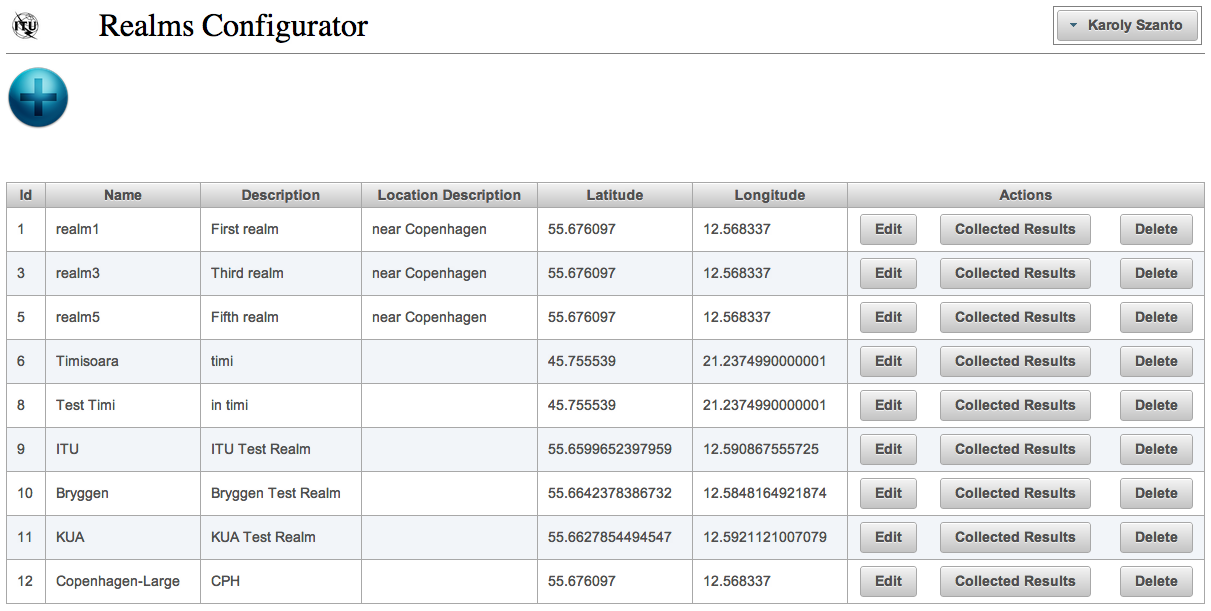
\includegraphics[width=\linewidth]{fig/my_realms.png}
	\caption{"My realms" view}
	\label{fig.my_realms}
\end{figure}

\noindent Figure \ref{fig.my_realms} depicts the home page of the configurator which presents the user with the realms he has created so far, if any. The user can choose to \emph{Create} a new realm, to \emph{Edit/Delete} an existing one or to see the \emph{Collected Results} (presents the persisted realm users feedback -- answers to questions or ratings for informations).
\\

\noindent By pressing the create new realm button (the "+" button) the user will be presented with the "Create Realm" page depicted in Figure \ref{fig.new_realm}. A search by address feature helps for easy navigation to the desired location described by a complete address, a city name, a symbolic location name (e.g IT University of Copenhagen) etc. To achieve the desired precision when placing the marker on the map, the user can use the zoom in and zoom out features to get a more/less detailed view and can drag the marker to another location. The radius of the realm (represented in meters) can be adjusted by modifying the appropriate input field. The realm radius is represented as a red circle around the marker. Once all the required data has been filled in, the user can save the newly realm.
\begin{figure}[H] 
	\centering
	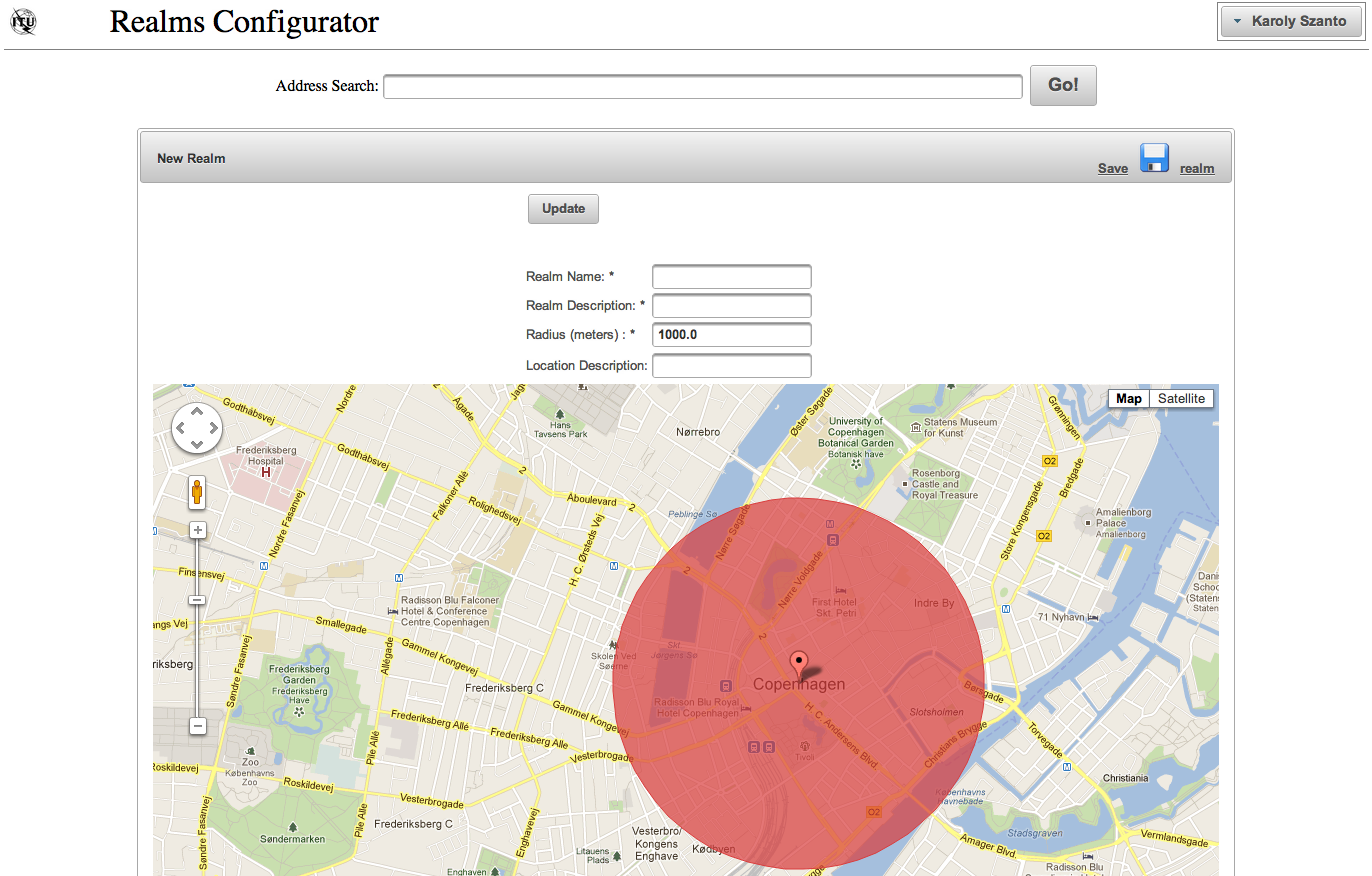
\includegraphics[width=\linewidth]{fig/new_realm.png}
	\caption{"Create Realm" view}
	\label{fig.new_realm}
\end{figure}
\\

\noindent Adding markers to a realm is supported in the "Configure Realm" page illustrated in Figure \ref{fig.edit_realm1}. This page can be reached either by saving a newly created realm in the create realm page or by choosing the edit realm option in the my\_realms page.
\begin{figure}[H] 
	\centering
	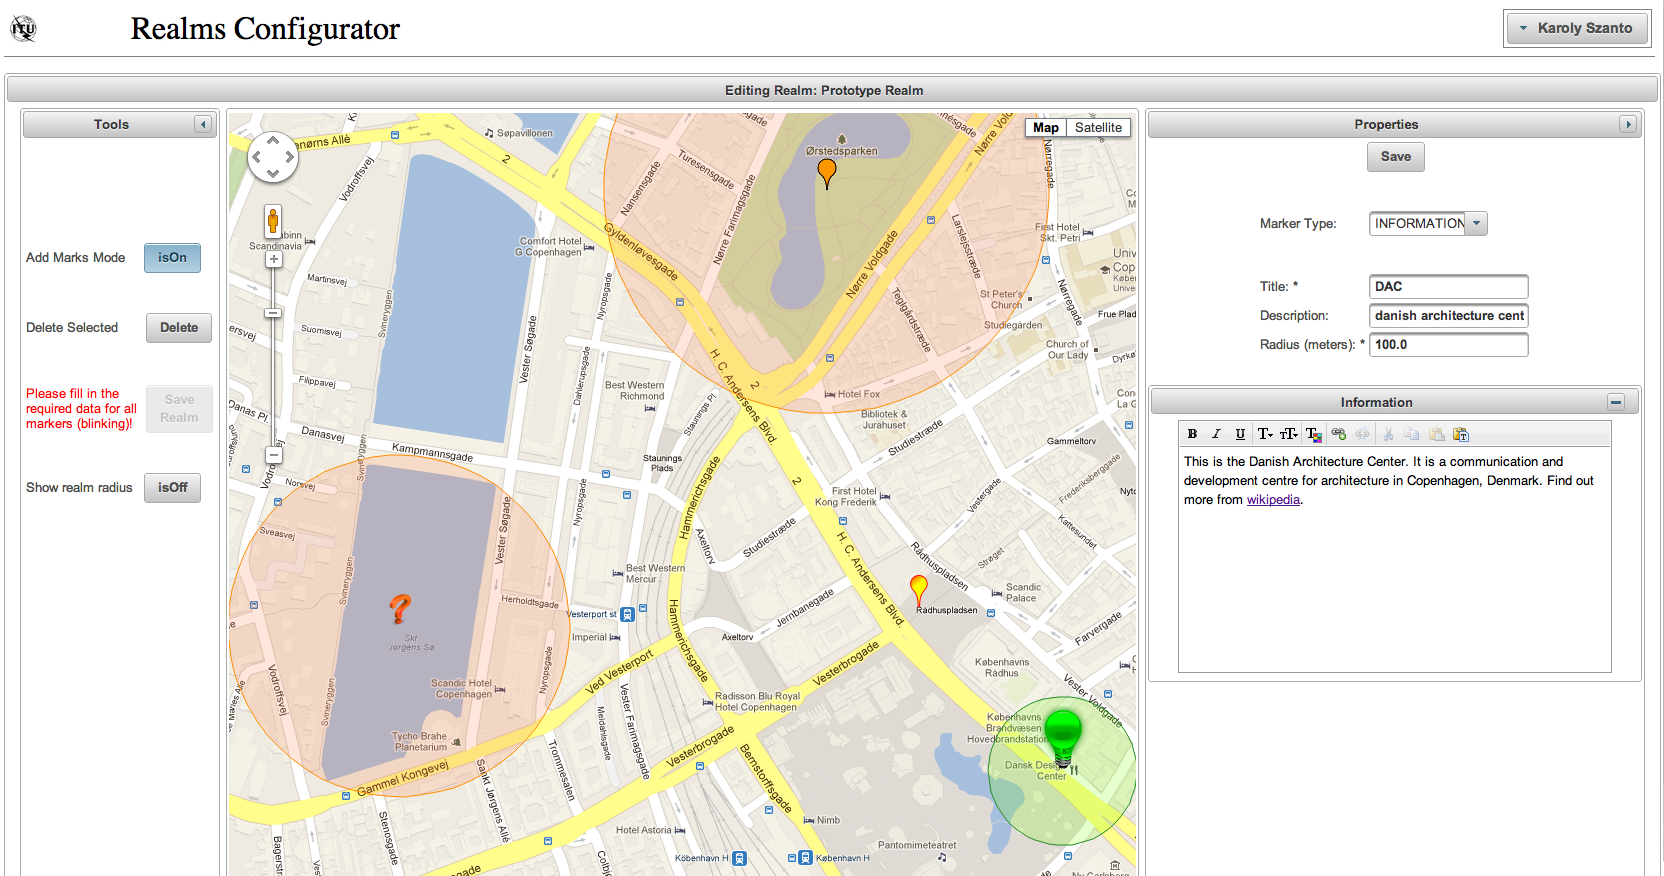
\includegraphics[width=\linewidth]{fig/edit_realm1.png}
	\caption{Edit Realm view with incomplete makers}
	\label{fig.edit_realm1}
\end{figure}
\noindent This page is made up by three different panes:
\begin{itemize}
	\item tools -- the left pane provides general tools to which help the configuration process
 	\item map -- the central pane provides a map on which markers can be placed
	\item properties -- the right pane allows editing the selected markers properties.
\end{itemize}

\noindent First we will describe each option provided by the tools pane:
\begin{itemize}
	\item Add marks mode -- enables or disables adding markers to the map. When this option is enabled, a simple click on the map will create add a new marker at that location.
	\item Delete selected -- deletes the selected marker. Only enabled if a marker is selected.
	\item Save realm -- save all the changes made so far and take the user back to the my\_realms page. This option is only enabled if all the required data for all the markers in the realms is filled in.
	\item Show realm radius -- toggle between displaying or hiding the circle representing the coverage area of this realm.
\end{itemize}

\noindent When markers are added to the map they don't have any data filled in by default. It is the users responsibility to configure each marker with the desired information. A marker can be configured as either an information or a question. Therefore, a marker can be in different states during a configuration process which requires different graphical representations to make the interaction intuitive and easy:
\begin{itemize}
	\item a marker that does not have all the required data filled in is represented as an inverted water drop with a blinking black dot in the middle
	\item an information marker is represented as a light bulb
	\item a question marker is represented as a question mark
	\item unselected markers are orange whereas the selected marker is green and double in size.
\end{itemize}

\noindent As mentioned before, the properties pane enables the user to edit the selected markers properties. The selected marker in Figure \ref{fig.edit_realm1} is configured to be an information marker (the required properties are title and radius). The information is typed into a an input element with rich text editing features. In Figure \ref{fig.edit_realms2} the selected marker is a question marker. The properties pane is slightly different -- instead of entering information the user can enter a question (in the same editor enabled with rich text editing features) together with a set of possible options to choose from. At most one of the options can be marked as an answer.
\begin{figure}[H] 
	\centering
	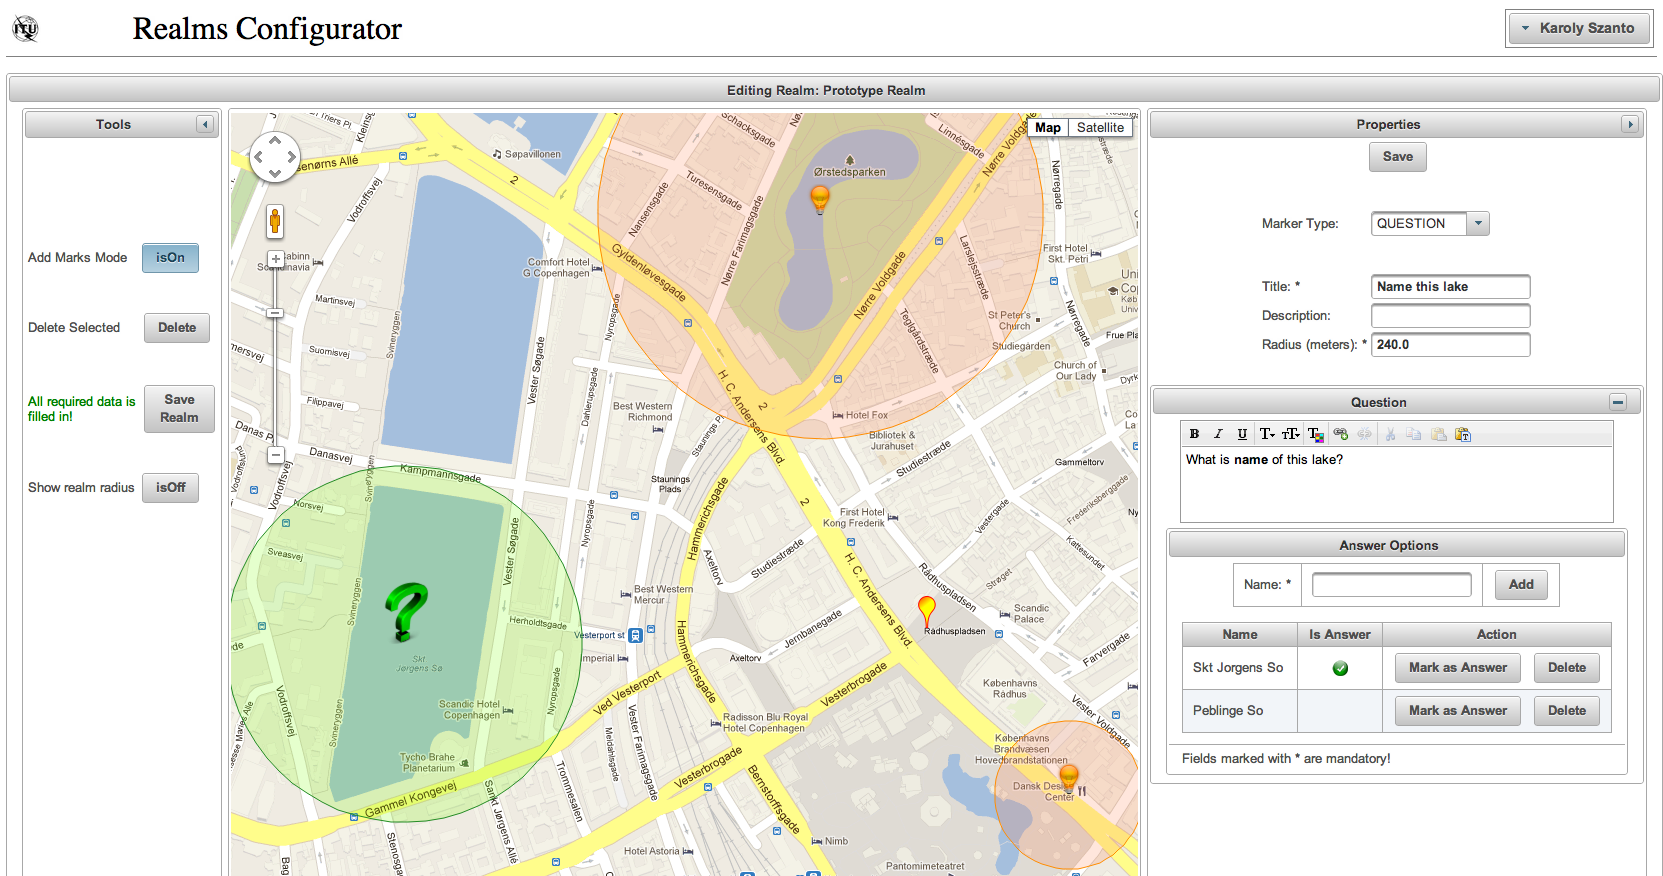
\includegraphics[width=\linewidth]{fig/edit_realm2.png}
	\caption{Edit Realm view with complete markers}
	\label{fig.edit_realm2}
\end{figure}

\noindent Finally, we would like to shortly describe the feedback page depicted in Figure \ref{fig.feedback} which presents the feedback collected from the realm users. As illustrated in the figure, each entry represents an individual feedback characterised by the user who submitted it, the marker it was submitted for and the user feedback. For an information marker the feedback is a rating ranging from 1-5 and for a question marker it is the select option (from the marker's set of possible options).
\begin{figure}[H] 
	\centering
	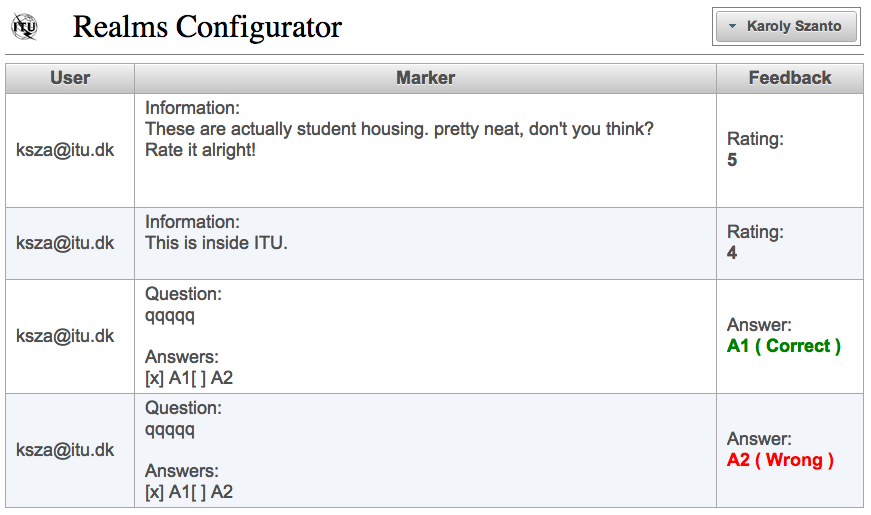
\includegraphics[width=\linewidth]{fig/feedback.png}
	\caption{Feedback page}
	\label{fig.feedback}
\end{figure}


\subsection{Realms Android App}
\noindent We have implemented the mobile client as an Adroid\footnote{http://www.android.com}. The application has to perform three main taks:
\begin{itemize}
	\item provide the most accurate location as long as the application is running
	\item carry out location-based and location-enhanced interactions with the server
	\item present the user with the results of the interactions
\end{itemize}

\noindent For data sensing we have used the Funf Open Sensing Framework\footnote{http://funf.media.mit.edu}. The Funf Open Sensing Framework is an extensible sensing and data processing framework for mobile devices, developed at the MIT Media Lab. We have chosen this framework because it provides built-in accurate location sensing making use of GPS, Wi-Fi and mobile network (GPRS tower cell ID) data to accurately locate the device. At application start-up we start funf's monitoring service. Each time we get a new reading, we store it in a local database -- we have configured funf to report location data sensed having an accuracy of at most 20 meters. This way the latest accurate location is available to be read by component of the application.
\\

\begin{figure}[H]
        \centering
        \subfigure[]{
                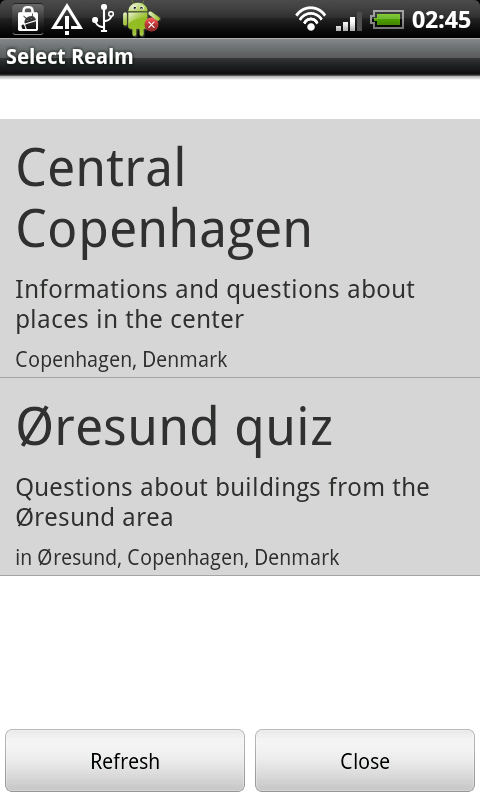
\includegraphics[width=0.3\linewidth]{fig/client/select_realm.png}
                \label{fig.client.select_realm}
        }
        \subfigure[]{
                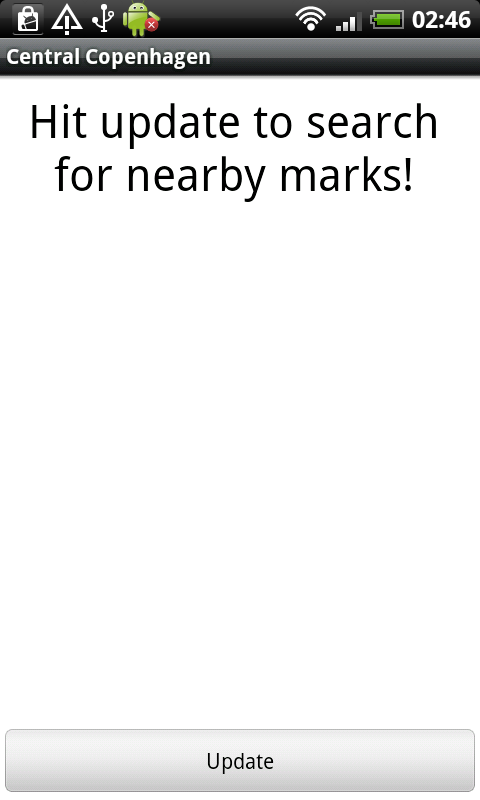
\includegraphics[width=0.3\linewidth]{fig/client/search_for_marks.png}
                \label{fig.client.find_markers}
        }
        \subfigure[]{
                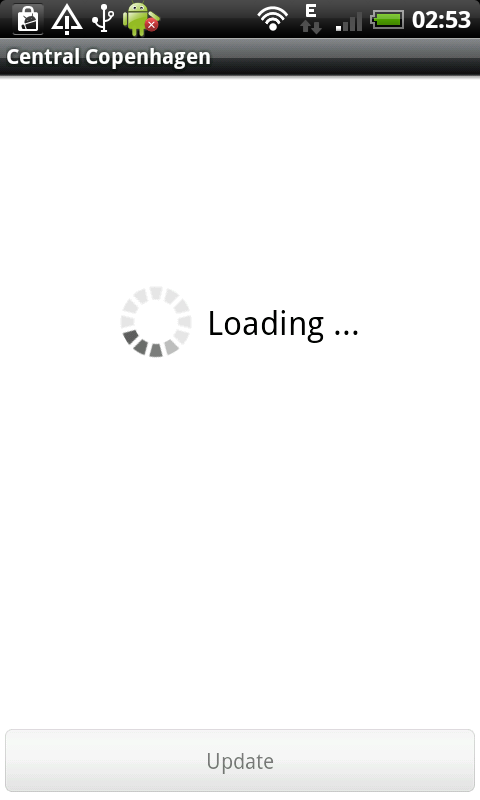
\includegraphics[width=0.3\linewidth]{fig/client/loading.png}
		\label{fig.client.loading}
        }
        \subfigure[]{
                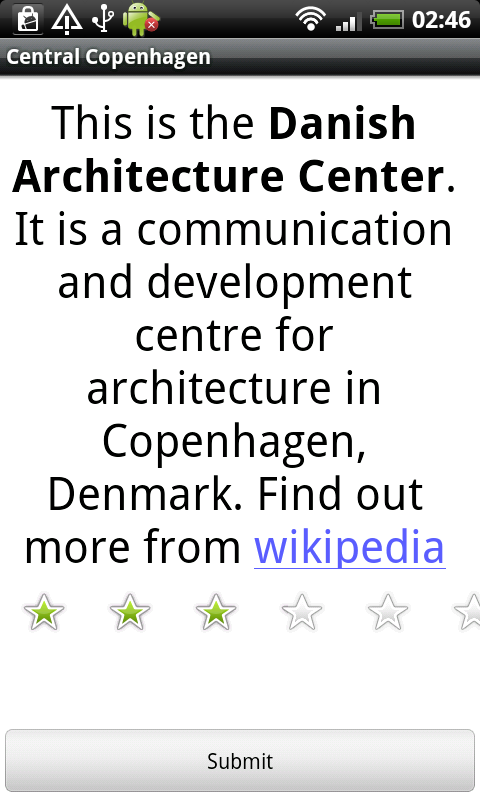
\includegraphics[width=0.3\linewidth]{fig/client/info_marker.png}
                \label{fig.client.info_marker}
        }
        \subfigure[]{
                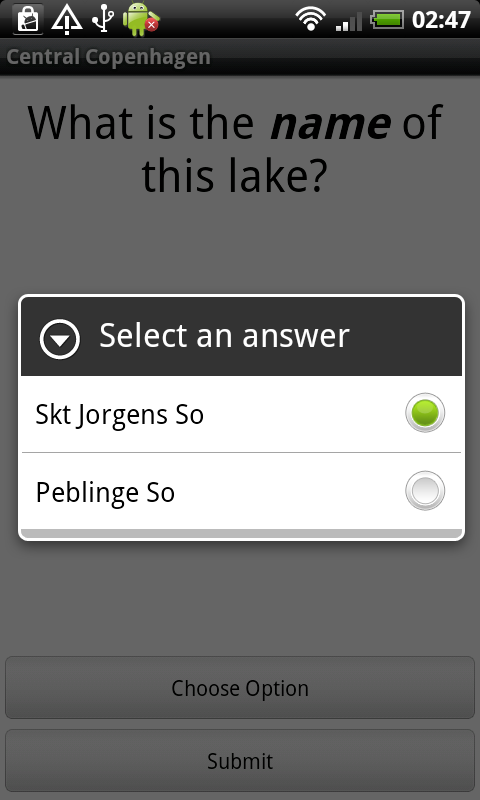
\includegraphics[width=0.3\linewidth]{fig/client/question_marker.png}
                \label{fig.client.question_marker}
        }
        \subfigure[]{
                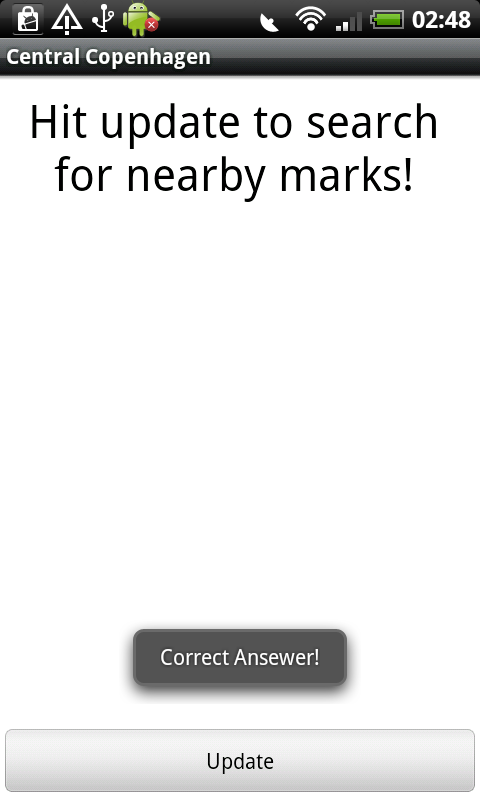
\includegraphics[width=0.3\linewidth]{fig/client/answer_feedback.png}
                \label{fig.client.answer_feedback}
        }
        \caption{The Realms Android App in action}
        \label{fig.client}
\end{figure}
\noindent Figure \ref{fig.client} depicts six screenshots of the working application which, in the followings, will help us discuss the implemented features. The first screen that is displayed to the user is the "select realm" screen illustrated in Figure \ref{fig.client.select_realm}. Once an accurate location reading is available the user can click the refresh button, action that will result in querying the server for the realms the user is currently in. A list of realms might be returned (if any) and presented to the user. Choosing one of the realms will take the user to a screen which enables the user to search for markers in the selected realm. Therefore, as depicted in Figure \ref{fig.client.find_markers} the user can query the server for nearby markers clicking on the Update button. It has to be noted that each communication with the server is time consuming and the user has to be informed about this. Figure \ref{fig.client.loading} illustrates a loading screen which we used to notify the inform the user about the long running operation every time a communication with the server is in process.
\\

\noindent After an update process the screen is populated with the marker data. For the information marker, illustrated in Figure \ref{fig.client.info_marker}, the formatted information data is displayed together with a rating bar rate the information in the marker. For the question marker, depicted in Figure \ref{fig.client.question_marker}, on the other hand, the screen displays the formatted question and a list of choices to choose an answer from. In both cases, information and question marker, a feedback will be selected and submitted to the server. After the submission is complete, the user will get feedback on the action he just completed. For rating an information the feedback is simply notifying the user about the chosen rating, whereas for answering a question will notify the user if the selected answer was correct or false, as depicted in Figure \ref{fig.client.answer_feedback}.
